%*************************************************************
\chapter{Design VS Computer}\label{ch:DesignVSComputer}
%*************************************************************

Wir arbeiten mit Dokumenten in zwei verschiedenen Welten: der elektronischen Welt des Computers und der physikalischen Welt am Schreibtisch. Jede Welt hat ihre Vor- und Nachteile (siehe \autoref{tab:wellnerDokumente}), welche uns dazu bewegen die >>richtige<< für bestimmte Aufgaben zu wählen \citep{Wellner:1993}.

\begin{table}
    \myfloatalign
\begin{tabularx}{\textwidth}{p{5cm}X}
    \toprule
	    \tableheadline{Elektronische Dokumente} & \tableheadline{Papierdokumente}
	     \\ \midrule
		\begin{itemize} 
			\item{schnell zum editieren}
			\item{schnelles kopieren}
			\item{schnelles senden}
			\item{schnelles freigeben}
			\item{schnelles ablegen}
			\item{schnelles abrufen}
			\item{erlaubt Stichwortsuche}
			\item{erlaubt \newline Rechtschreibprüfung}
			\item{erlaubt sofortige \newline Berechnungen}
		\end{itemize} &
		\begin{itemize} 
			\item{3-dimensional}
			\item{überall akzeptiert}
			\item{billig}
			\item{portabel}
			\item{geläufig}
			\item{hochauflösend}
			\item{einfach zu lesen}
			\item{fühlbar}
			\item{man kann beide \newline Hände \& Finger \newline zum bearbeiten \newline verwenden}
			\item{man kann mit einem Stift darauf kritzeln}	
		\end{itemize}
	\\  \bottomrule
\end{tabularx}
  \caption[Elektronische Dokumente und Papierdokumente \newline \citep{Wellner:1993}]{Gegenüberstellung der Eigenschaften von elektronischen Dokumenten und Papierdokumenten.}
  \label{tab:wellnerDokumente}
\end{table}

\begin{figure}
        \myfloatalign
        \subfloat[Geschriebene Darstellung (in der Wortebene).]
        {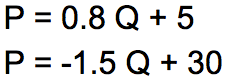
\includegraphics[width=.48\linewidth]{gfx/johnsonDarstellungsformenB}} \quad
        \subfloat[Graphische (schematische) Darstellung.]
        {\label{fig:johnsonDarstellungsformenB}%
         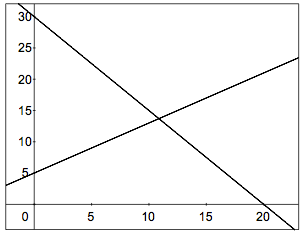
\includegraphics[width=.48\linewidth]{gfx/johnsonDarstellungsformen}} \\
        \caption[Darstellungsformen \newline \citep{Johnson:2009}]{Die schematische Darstellung (a) und die Darstellung in der Wortebene (b) eines mathematischen Verhältnisses. Beide Darstellungsformen zeigen die gleiche Information. }\label{fig:johnsonDarstellungsformen}
\end{figure}

\medskip In mancher Hinsicht scheint es aber, als wäre Papier bald obsolet. Manche prophezeien das papierlose Büro schon in wenigen Jahren. Das Eigenartige dabei ist nur, dass sich die Leute ungern von Papier trennen. Studien belegen, dass der Papierkonsum in Büros seit 1970 um das 6-fache anstieg und derzeit jährlich um 20\% steigt \citep{seybold:1992}. Papier hat ebenso wie elektronische Dokumente Eigenschaften, die Menschen nicht aufgeben wollen. Das macht sie in Hinsicht auf computerbasierende Alternativen >>unverwüstlich<<. \citep{Luff:1992} 

\medskip Wie wichtig Papier (im Zusammenhang mit Skizzen) für Designer ist, wurde auch im Kapitel \nameref{ch:designTheorie} beschrieben. Welchen Umstand dies das alte Medium zu verdanken hat, lässt sich laut Sellen und Harpers Arbeit \emph{The Myth of the Paperless Office} \citep{Sellen:2003} nicht durch einfache Merkmalgegenüberstellungen herausfinden. Nur Studien und Observationen können das kognitive Verhalten bei der Benutzung von Papier und digitalen Artefakten beschreiben. 

\medskip Das nun folgende Kapitel soll die Stärken und Schwächen traditioneller und digitaler Arbeitsweisen gegenüberstellen und mittels verschiedenster Studien eine Erklärung zum oben genannten Phänomen finden. -- Können die beiden Welten von einander lernen?
%Deswegen initierten Terrenghi et al. eine Designstudie, die dabei helfen sollte, das kognitive Verhalten bei der Benutzung von Papier und digitalen Artefakten zu beschreiben. \citep(Terrenghi:2007) Ihre Ergebnisse sollen in den nächsten beiden Abschnitten erläutert werden.

\section{Skizzieren auf Papier}
%Skizzieren erlaubt Personen mit abstrakten und ungenauen Elementen zu arbeiten, diese daraus resultierenden oft mehrdeutigen Kritzeleien wiederholt zu interpretieren und alternative Bedeutungen zu erlangen. Skizzierte Abbildungen, Bilder und Karten helfen Personen ihre Gedanken zu manifestieren oder Ideen anderen zu erklären. \citep{YiLuenDo:2005}
Skizzieren fördert eine schnelle und formlose Informationsverarbeitung. Wir würden z.B. eine Telefonnummer eher auf ein Whiteboard in der Nähe des Schreibtischs schreiben, als sie in den Computer einzugeben; bzw. schnelle Berechnungen oder \emph{To-Do-Lists} auf einem Blatt Papier, da sie leicht zu erstellen sind und das Ergebnis portabel ist.
Larkin und Simon verglichen \emph{schematische} Darstellungen mit \emph{Darstellungen in der Wortebene} (geschrieben oder gesprochen) und zeigen damit dass räumliche Darstellungen oft mehr aussagen als die gleiche Information in einem ausführlich geschriebenen Statement \citep{Larkin:1987}. Wie effizient Information verarbeitet werden kann hängt - technisch betrachtet - davon ab wieviel >>Rechenaufwand<< von Nöten ist, um Vorgaben so zu übersetzen damit Verständnis entsteht. Um beispielsweise einen mathematischen Ausdruck eines Verhältnisses zu beschreiben, würde sich eine schematische Darstellung besser eignen. Der gleiche Ausdruck als Darstellung in der Wortebene würde eine längere Berechnungszeit benötigen (siehe \autoref{fig:johnsonDarstellungsformen}).

\medskip Wenn Personen skizzieren, fassen sie relevante Informationen zusammen und lassen die irrelevanten aus \citep{Tversky:2002}. Zeichnen erlaubt Personen Papier als externen Speicher zu verwenden, um ihre kognitive Belastung zu verringern. Schematische Darstellungen stellen ein vereinfachtes Abbild von Informationsbereichen dar \citep{Tversky:2000}. Per Hand gezeichnete Landkarten bzw. Wegbeschreibungen zum Beispiel, werden üblicherweise mit simplen Formen wie Rechtecke oder Kreise für Gebäude, Linien oder Pfeile für Wege und sich überschneidende Linien für Kreuzungen gezeichnet \citep{Tversky:1999}. Die Form und Krümmung von Gebäuden und Linien werden lediglich geschätzt, da Menschen bei genau gezeichneten Karten hingegen Schwierigkeiten haben, die kleinen Unterschiede zwischen der Karte und der echten Welt abzugleichen. Räumliche Darstellungen sind ebenso ein beeindruckendes Hilfsmittel beim Lernen. Skizzieren erlaubt Lernenden Konzepte, so wie sie verstanden wurden, aufzuzeichnen und diese von erfahrenen Personen auf Inkonsistenzen und Fehlern zu überprüfen \citep{Forbus:2008}.
%Van Sommers studierte ausgiebig das Zeicheinverhalten von Personen \citep{VanSommers:1984}. 

\medskip Goel führte in \citep{Goel:1995} eine Reihe an Experimenten durch, um die kognitiven, handlungsauffordenrnden Merkmale von Skizzen zu erforschen. In seinen Studien verglich er traditionelle Papier-und-Stift Skizzen mit Skizzen, die mit Hilfe von computerbasierten Zeichenprogrammen erstellt wurden. Die teilnehmenden Designer bekamen Anweisungen ein Artefakt auf beide Arten zu designen. Dabei kam ein modifiziertes Softwaretool zum Einsatz, das lediglich strukturierte Eingaben, wie gerade Linien, Rechtecke und Ellipsen unterstützte. \graffito{Skizzieren mit einem strukturierten Softwaretool kommt nicht an die Schnelligkeit von unstrukturierten Papier-und-Stift Skizzen heran.} Die Ergebnisse zeigten, dass das strukturierte Computerprogramm bezüglich der Ideenfindung, nicht an die Schnelligkeit vom unstrukturierten Papier-und-Stift System herankam. Skizzieren unterstützt Designer bei der schnellen Entwicklung vieler unterschiedlicher Ideen. Diesen explorativen Charakter von Skizzen beschrieb Goel als \emph{Quertransformationen}, die sich im Gegensatz zu den \emph{vertikalen Transformationen}, welche sich durch Verfeinern von Ideen auszeichnen, deutlich abgrenzen. Bei den beiden Transformationstypen stützt sich Goel auf die von Newman und Landay in \citep{Newman:2000} beschriebenen Aktivitäten verschiedener Designstufen. Am Anfang des Designprozesses sind Designer mit der Ideengenerierung und -findung beschäftigt (Quertransformationen). Später konzentrieren sich Designer schrittweise Überarbeitungen und Änderungen (vertikale Transformationen).

\medskip 

\section{Skizzieren am Computer}

Heutige stiftbasierte Hardware orientiert sich vorwiegend am Schreiben und Lesen von Text. Wenn man erwägt diese auch für Designaktivitäten einzusetzen, sollte man sie mit den Werkzeugen, die Designer in der Praxis benutzen vergleichen. \\ Designer können schnell Zeichnungen auf Papier anfertigen und zwischen den einzelnen Seiten blättern. Sie können ebenfalls die Zeichnungen nebeneinander an die Wand heften, um sie zu vergleichen. Die Stiftspitze zeichnet dabei sofort bei Berührung auf dem Papier und es können zwei Hände benutzt werden um das Blatt Papier nach Belieben zu drehen bzw. um Hilfsmittel wie ein Lineal zu halten.

\medskip Am einfachsten wäre es, wenn computerunterstützes Skizzieren genau die selben Eigenschaften aufweisen würde. Jedoch mangelt es der derzeitigen Hardware an Portabilität, schnellem Reaktionsvermögen und dem vertrauten Gefühl traditioneller Designpraktiken. Die kommerzielle Entwicklung und Forschung verbessert kontinuierlich Hardware auf diesem Sektor, so unterstützen viele Geräte wie z.B. PDAs, Tablet PCs oder interaktive Wandinstallationen bereits eine Art von Stift- oder Touchinput. Während stiftbasierte Systeme seit Jahrzehnten bei Forscher im Einsatz sind, verbreiten sie sich erst seit Mitte der 90er Jahre und werden stetig billiger.

\medskip >>Skizzierhardware<< kann in zwei Gruppen unterteilt werden: 
\begin{itemize}
	\item{Hardware, die nur Eingaben unterstützt, und}
	\item{Hardware, die Eingaben und Ausgaben unterstützt.}
\end{itemize}

Tablets geben den Benutzern die Möglichkeit mit Hilfe eines Eingabestifts zu schreiben bzw. zu zeichnen. Manche beschränken sich dabei aber lediglich auf die Eingabe und zeigen nicht gleichzeitig das Gezeichnete. Geräte, die Ein- und Ausgaben unterstützen, haben sich besonders bei den Tablet PCs durchgesetzt. Zusätzlich gibt es auch Systeme, die das gezeichnete indirekt >>scannen<<. Z.B. entwickelte PARC das ScanScribe System, welches Zeichnungen analysiert, die mit herkömmlichen Stift und Papier erzeugt wurden und erstellt daraus eine mit dem Computer aufgebesserte Version. \citep{Johnson:2009}

\subsection{Electronic Ink}
Wenn man eine Zeichnung mit künstlerischem Ausdruck zu Papier bringt, gibt es viele Faktoren die das Endergebnis beeinflussen. So z.B. die Stärke des Schreib- bzw. Zeichengeräts, sowie die Materialeigenschaften des Papiers. In vielen Branchen, wie beispielsweise in der Computeranimation, ist es noch immer üblich Illustrationen zuerst auf Papier zu zeichnen und danach schrittweise zu digitalisieren. Es wurden zwar einige Versuche gestartet direkt auf digitaler Ebene zu zeichnen, jedoch wird dies nach wie vor hauptsächlich nur dort verwendet, wo der Computer nicht nur optional benutzt wird. \citep{Henzen:2005}

Viele Tablets sind Druckempfindlich. Designer benutzen oft stärkere Linien um Objektgrenzen hervorzuheben und dünne Linien um dezente Texturen, Schatten oder Rundungen anzudeuten. Geräte, die Druck messen können, erlauben Designer dickere oder dunklere Striche zu zeichnen, ohne vorher in einen anderen Zeichenmodus wechseln zu müssen.

Die Druckmessung wurde auf verschiedene Weisen umgesetzt. Z.B. durch zwei übereinander liegenden leitfähigen Schichten mit entgegengesetzten Stromrichtungen. Die Schichten berühren sich nicht und sind oft durch eine nicht leitende Flüssigkeit abgeschirmt. Wenn etwas (ein Stift oder Finger) die obere Schicht berührt, verändert sich die Spannung und die Position kann mittels Interpolation an den Kanten errechnet werden. Andere berührungsempfindliche Oberflächen messen die elektrischen Eigenschaften der Dinge, die sie berühren -- darum funktionieren auch Handschuhe auf manchen Laptop Trackpads nicht. Wacom\texttrademark{} Tablets und gleichartige induktive Geräte, benötigen spezielle Stifte, die in einem vom Tablet generierten elektromagnetischen Feld mitschwingen. Wieder andere Tablets erkennen akkustische oder optische Störungen zur Positionsberechnung.

Es gibt Oberflächen, die lediglich die Koordinaten eines einzigen Berührungsortes liefern können und Oberflächen die mehrere erkennen - auch Multitouchoberflächen genannt. Multitouchsysteme, wie z.B. \emph{Hans's Frustrated Total Internal Reflection technique} \citep{Han:2005} und \emph{Microsoft's Surface System} \citep{Surface:2010} befinden sich derzeit im Aufschwung, werden aber mit den Fingern order Händen benutzt und bieten deswegen völlig andere Anwendungserlebnisse als Stiftbasierte Oberflächen.

\subsection{Der Unterschied zwischen Eingabestift und Maus}

Egal welche Abtasttechnologie man wählt, alle oben genannten Geräte erlauben Benutzern eine Eingabevariante, die näher an das traditionelle Schreiben herankommt, als die Maus jemals könnte. Obwohl Stift- und Mauseingaben viele Eigenschaften teilen (beide erlauben Benutzer im 2D Raum zu interagieren), haben sie einige grundlegende Unterschiede.

\medskip Mauseingaben liefern Daten über die \emph{Bewegung} - und Stifteingaben liefern Daten über die \emph{Position} \citep{Hinckley:2002}. Mit anderen Worten produzieren Mäuse relative \emph{Änderungen} in der (x,y) Position und Stifte direkte, absolute (x,y) Positionen. Benutzer können Tablets aber auch so konfigurieren, damit sie sich wie Mäuse verhalten und relative Positionen erzeugen.

\medskip Die Form der Geräte ist ebenfalls extrem wichtig. Ein Stift zwingt die Benutzer die Feinmotorik ihrer Finger einzusetzen um die Stiftspitze zu steuern, wohingegen die Hand- und Unterarmmuskeln die Maus steuern. Finger können zwar auch zur Maussteuerung benutzt werden, aber nicht mit der gleichen Fertigkeit. Je nach Art der Arbeit, ist ein Stift ergonomisch besser als eine Maus - oder umgekehrt.

Tablets können aber mehr als nur die Stiftposition erkennen. Manche Geräte können auch den Aufpressdruck, den Winkel oder die Rotation des Stifts messen. Das andere Ende des Stifts wird auch oft als alternativer Modus (z.B. als ein Radierer) benutzt. 

Einige Stifte haben noch zusätzliche Buttons. Während Buttons unentbehrliche Bestandteile von Mäusen sind, können sie entlang des Stiftgehäuses schwer benutzbar sein \citep{Plimmer:2008}. Die Kraft, die bei einem Buttonklick an der \emph{Maus} entsteht, ist orthogonal zu der Oberfläche, auf der die Maus benutzt wird und beeinflusst die Zielgenauigkeit nur unwesentlich. Ein Knopfdruck am \emph{Stift} hingegen, kann die Stiftspitze ungewollt bewegen, was das Zeigen auf ein \graffito{Buttons an Tabletstiften können schwer benutzbar sein und sich auf längere Zeit unangenehm auswirken.}bestimmtes Objekt und das gleichzeitige Drücken einer Taste erschwert (siehe \autoref{fig:johnsonButtonPress}). Zudem muss der Benutzer beim Drücken einer Taste üblicherweise den Stift erst so drehen, damit sich sein Finger wieder über der Taste befindet (was durchaus öfter vorkommt). Diese Aktion lenkt ab und ist auf längere Zeit gesehen unbequem. \citep{Johnson:2009}

\begin{figure}
        \myfloatalign
        \subfloat[Drücken einer Maustaste erzeugt eine Kraft, die orthogonal auf die darunterliegende Oberfläche wirkt.]
        {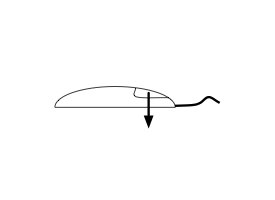
\includegraphics[width=.48\linewidth]{gfx/johnsonMousePress}} \quad
        \subfloat[Drücken einer Stifttaste erzeugt eine ungewollte Stiftspitzenbewegung.]
        {\label{fig:johnsonButtonPressB}%
         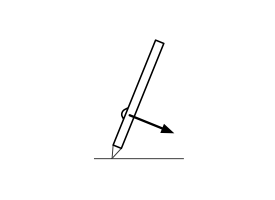
\includegraphics[width=.48\linewidth]{gfx/johnsonStylusPress}} \\
        \caption[Kräfte bei Buttonklicks. \newline \citep{Johnson:2009}]{Entstehende Kräfte beim Drücken einer Maustaste (a) und einer Stifttaste (b) eines Tablets.}\label{fig:johnsonButtonPress}
\end{figure}

\subsection{Interaktionstechniken für stiftbasierte Skizziersysteme} %5.5
Bei der Entwicklung neuer Technologien ist es wichtig das Ausmaß der kognitiven Belastung des Tools zu berücksichtigen. Aus Oviatt's Studie \citep{Oviatt:2006} über Mathematikstudenten geht hervor, dass das Arbeiten mit stiftbasierte Applikationen auf Tablet PCs erheblich schlechter funktioniert als mit herkömmlichen Stift und Papier. Durch die Benutzung der Tablets benötigten die Studenten mehr Zeit bei der Lösung von Mathematikaufgaben, was dazu führte dass sie sich mit der Technologie nicht anfreunden konnten. Anthony et al. führten eine ähnliche Studie durch, in der sie Eingaben von Studenten verglichen, die Gleichungen beinhalteten. Zur Eingabe dienten ein \emph{Standard \acs{WIMP}\footnote{Die Abkürzung WIMP wurde 1980 von Merzouga Wilberts ins Leben gerufen und steht für Window, Icon, Menu, Pointing Device. Es bezeichnet das Grundkonzept moderner grafischen Benutzerschnittstellen (\acp{GUI}).} Interface} und ein Eingabetablet \citep{Anthony:2005}. \\ Sie kamen zur Erkenntnis, dass die Studenten Stifteingaben bevorzugten und \graffito{Umso mehr Aufmerksamkeit man (Software-)Tools schenken muss, desto weniger Aufmerksamkeit bekommt das eigentliche Problem.}handgeschriebene Gleichungen schneller und genauer niederschreiben konnten, als mit Keyboard und Maus. Papier und Stift wurden dem elektronischen Schreiben zwar vorgezogen, jedoch waren ihnen Stifte im Allgemeinen lieber als Tastatur- und Mauseingaben. Beide Studien kamen zum selben Schluss: Je mehr Aufmerksamkeit Benutzer aufbringen müssen um das Tool zu verwenden, desto weniger Aufmerksamkeit schenken sie dem eigentlichen Problem.

\medskip Zur Redzuierung der kognitiven Belastung müssen demnach natürlichere Interaktionstechniken entwickelt werden. Verschiedenste Methoden erwiesen sich bis dato durchaus brauchbar zum effizienten Arbeiten mit Stiftapplikationen. Kontextmenüs sind ein gutes Beispiel dafür \citep{Kurtenbach:1991}. Traditionelle Menüs zeigen eine Liste an Optionen, welche das Menü nach unten und rechts wachsen lassen. Bei Tablets, die Eingaben und Ausgaben unterstützen (z.B. Tablet PCs) kann dies dazu führen, dass Benutzer das Menü mit der Hand verdecken. >>Torten<<-Menüs (eine Art Kontextmenü) erscheinen zentriert um die Stiftposition und zeigen die Optionen kreisförmig (siehe \autoref{fig:johnsonPieMenu}). Die Hand ist zwar bei dieser Art von Menüs noch immer teilweise im Weg, aber zumindest ist ein Teil des Menüs dadurch sichtbar. Der Vorteil dieser Methode ist, dass sich Personen Gesten anlernen können, ohne die Menüeinträge jedesmal erneut lesen zu müssen. Vorraussetzung dafür ist jedoch, dass sich die Menüeinträge niemals ändern. Eventuell schwindet auch der Bedarf eines visuellen Menüs durch die Gesten. Tortenmenüs werden in Applikationen wie Maya \citep{Maya:2010}, Spielen wie The Sims \citep{EA:2010} oder als Erweiterungen in Webbrowser verwendet. Der Ansatz funktioniert zwar gut, bringt aber auch zwei Nachteile mit sich. Zum einen ist es nicht klar wie man das Menü aufrufen kann und zum anderen müssen Gesten erst entdeckt, erlernt und ins Gedächtnis gerufen werden.

\begin{figure}
        \myfloatalign
        \subfloat[Tortenmenüerweiterung für den Firefox Webbrowser.]
        {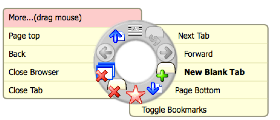
\includegraphics[width=.48\linewidth]{gfx/johnsonPieMenuFF}} \quad
        \subfloat[Autodesk Maya Tortenmenü.]
        {\label{fig:johnsonPieMenuB}%
         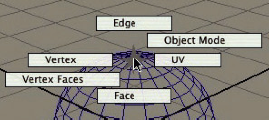
\includegraphics[width=.48\linewidth]{gfx/johnsonPieMenuMaya}} \\
        \caption[Tortenmenüs \newline \citep{Johnson:2009}]{Tortenmenüs in Firefox (a) und Maya (b).}\label{fig:johnsonPieMenu}
\end{figure}

\medskip Ramos et al. \citep{Ramos:2004} erforschte weiters die Benutzung von Aufpressdruckdaten bei stiftbasierenden Interaktionen. Zu der zweidimensionalen (x,y) Stiftposition kommt die Druckstärke des Stiftes als dritte Dimension hinzu, die der Benutzer frei verändern kann. Zum Beispiel kann ein leichter Druck ein Menü zeigen und ein harter Druck ein anderes Menü. Druck kann eine effektive Eingabeart sein, wenn sie richtig (mit haptischen und visuellen Feedback) eingesetzt wird.

\medskip Hinckley et al. \citep{Hinckley:2005} empfiehlt die Benutzung von \emph{Begrenzer} um Kontextmenüs aufzurufen. \emph{Begrenzer} sind Eingaben, die Benutzer normalerweise nicht zeichnen würden aber dennoch leicht zu merken sind. Ein Beispiel zeigt ihr System Scriboli, in dem ein >>Rattenschwanz<< (eine Schleife am Ende einer Selektionsgeste) als Begrenzer benutzt wird. Diese flüssige Bewegung lässt den Benutzer Zielobjekte kennzeichnen um auf sie anschließend ein Kommando anwenden zu können.

\medskip Wieder andere haben Interface Idiome\footnote{Ein Idiom im Sinne der Softwaretechnik ist ein programmiersprachenspezifisches Muster. Ein Idiom beschreibt, wie man bestimmte Aspekte von Komponenten oder Beziehungen zwischen ihnen mit den Mitteln einer bestimmten Programmiersprache implementiert \citep{Buschmann:1998}.} zur Unterstützung von Stift- \& Skizzeneingaben entwickelt. \emph{Gedrics} sind auf Gesten basierende Icons für stiftbasierte Applikationen \citep{Geissler:1995}. Jedes Gedric ist mit einer Klasse an Aufgaben, wie >>ändere die Schriftarteigenschaften<< in einem Texteditor, verknüpft. Um ein Kommando durchzuführen, muss der Benutzer eine Geste auf ein Gedric zeichnen. Das System erkennt die Geste und gibt dem Icon anschließend die auf die Geste verknüpfte Bedeutung, welche durch Darauftippen aktiviert wird. Zeichnet man z.B. eine schräge Linie auf einem >>Schriftart<<-Gedric stellt das System einen markierten Text kursiv. Zeichnet man eine vertikale Linie von unten nach oben, wird die Schriftgröße erhöht. \\ So komfortabel Operationen auf Gedrics auch wirken, erfordern sie trotzdem eine Eingewöhnungsphase, in der Benutzer lernen müssen ihre Absichten in Gesten umzuwandeln. (vgl. \autoref{fig:geisslerGedric}) 

\begin{figure}
        \myfloatalign
        \subfloat[Gedric Icons.]
        {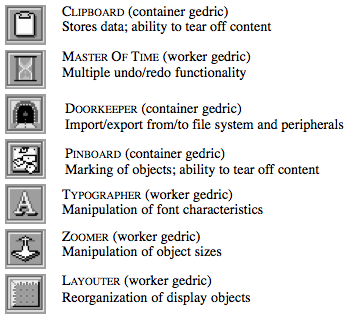
\includegraphics[width=.38\linewidth]{gfx/geisslerGedricIcons}} \quad
        \subfloat[Layouter Gesten.]
        {\label{fig:geisslerGedricIcons}%
         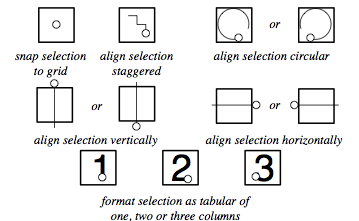
\includegraphics[width=.58\linewidth]{gfx/geisslerGedricLayouter}} \\
        \caption[Gedric \newline \citep{Geissler:1995}]{Beispiele für Gedric Icons (a) und Gesten einer Layoutfunktion (b).}\label{fig:geisslerGedric}
\end{figure}

\medskip Während Point \& Click Aktionen für Aufgaben zu Anwendungen, die üblicherweise mit der Maus ausgeführt werden ausgelegt sind, raten Accot und Zhai zur \emph{Kreuzen}-Technik zur Stiftinteraktion \citep{Accot:2002}. Das experimentelle Zeichenprogramm \emph{CrossY} \citep{Apitz:2004} zeigt Interface Widgets\footnote{Widgets (dt. Steuerelemente) sind Interaktionselemente in einer grafischen Benutzeroberfläche (\ac{GUI}), beispielsweise eine Schaltfläche oder eine Bildlaufleiste.}, die Kreuzen erlauben. Um ein CrossY Button zu aktivieren, muss der Benutzer eine Linie von einer Seite des Buttons zur anderen zeichnen, und somit den Button überqueren. Kreuzen macht es möglich mehrere Aktionen in einer flüssigen Bewegung abzuhandeln. Zum Beispiel kann man die Farbe und Stärke der Electronic Ink des Stiftes gleichzeitig ändern, in dem man den Stift über benachbarte CrossY Widgets bewegt (siehe \autoref{fig:accotCrossY}).

\begin{figure}[bth]
	\begin{center}
	
	{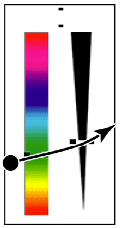
\includegraphics[width=0.3\linewidth]{gfx/accotCrossY}}
	\caption[CrossY \newline \citep{Johnson:2009}]{CrossY Interface Widgets erlauben Benutzer mehrere Parameter mit einer einzigen Bewegung zu ändern -- in diesem Beispiel die Stiftfarbe und -stärke.}
	\label{fig:accotCrossY}
	\end{center}
\end{figure}

\medskip So wie Skizzen mehrdeutig sein können, können auch stiftbasierte Interaktionen, wie das Drücken eines Buttons oder die Auswahl eines Menüpunktes, mehrdeutig sein. Wenn der Benutzer mit Hilfe des Stiftes, mit einem Objekt interagieren will, kann es sein, dass das System sein Ziel erst eindeutig machen muss. Zum Beispiel kann beim Drücken eines Buttons der Stift unabsichtlich zu einem anderen Button rutschen. Dieser Umstand wird auch \emph{Target Amibiguity}, oder laienhaft übersetzt \emph{Ziel Mehrdeutigkeit} genannt \citep{Mankoff:2000p77,Mankoff:2000}. \\
Eine Alternative um gegen die Mehrdeutigkeit vorzugehen, ist sie im Voraus zu bekämpfen. Pegasus und Chateau demonstrieren in \citep{Igarashi:2001,Igarashi:2003} ein \emph{Empfehlungssystem}, das vorhersagt was der Benutzer zeichnen wird und alle möglichen Aktionen aufzeigt. Diese Technik eignet sich besonders, wenn die Umgebung eine regelmäßige Grammatik aufweist oder strukturierte Eigenschaften wie Symmetrie genutzt werden soll.
Tsang et al. benutzten ein Empfehlungssystem in ihrem Programm, das Formen wie Flugzeugaußenhüllen modellieren kann \citep{Tsang:2004}. Das System bietet ein Overlay, das den Benutzer durch zusätzlichen Skizzierinput leitet. Benutzer zufolge führt dies zu präziseren Input. Das System benutzt die angefangenen Skizzen als Vorlagen, vergleicht diese mit Datenbankeinträgen um ähnliche Zeichnungen zu finden und empfielt zusätzliche Geometrie, die vielleicht dazu passen könnte.

\medskip Bae's 3D Kurvenmodellierungsystem zeigt wie verschiedene kaligraphische Interaktionstechniken zusammen benutzt werden können um eine flüssige Skizzierumgebung zu schaffen \citep{Bae:2008}. Das sog. \emph{ILoveSketch} System imitiert ein physikalisches Skizzierbuch. Die Eingaben erfolgen per Stift und können optional durch drücken von physikalischen Buttons durch die andere Hand verändert werden (siehe \autoref{fig:baeILoveSketch}). Das Interface verzichtet auf herkömmliche on-screen Buttons, Scrollbars und Menüs. Stattdessen gibt der Benutzer Kommandos durch Gesten, die oft vom Kontext abhängen. Zum Beispiel kann der Benutzer zu älteren Zeichnungen zurück >>blättern<<, in dem er an einer Ecke zieht. Um ein Objekt zu löschen, muss der Benutzer eine >>Durchstreichen<<-Geste anwenden. Viele Techniken in ILoveSketch betreffen Herausforderungen beim Skizzieren von 3D Objekten. Zum Beispiel errechnet das System automatisch aus der Arbeit des Benutzers die richtige Blickrichtung durch Drehungen und Verschiebungen.

\begin{figure}[bth]
	\begin{center}
	
	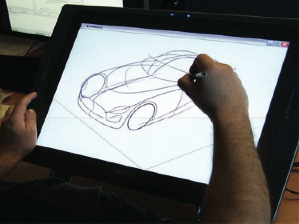
\includegraphics[width=0.7\linewidth]{gfx/baeILoveSketch}
	\caption[ILoveSketch \newline \citep{Johnson:2009}]{ILoveSketch zeigt ein >>natürliches<< Skizziersystem, welches mehrere kaligraphische Interaktionstechniken miteinander vereint \citep{Bae:2008}.}
	\label{fig:baeILoveSketch}
	\end{center}
\end{figure}

Alvarado fasste in \citep{Alvorado:2004} eine Liste aus sieben Designguidelines zur Entwicklung von \emph{Sketch Recognition User Interfaces} (Benutzeroberflächen zur Skizzenerkennung), kurz SkRUIs zusammen: 

\begin{enumerate}
	\item Zeige Skizzenerkennungsergebnisse erst wenn der Benutzer fertig ist mit dem Zeichnen
	\item Sorge für offensichtliche Hinweise um das Skizzieren von der Erkennung zu unterscheiden
	\item Beschränke die Erkennung auf einen einzelnen Bereich, solange keine automatische Bereichserkennung machbar ist
	\item Integriere stiftbasiertes Editieren
	\item Skizzieren und Editieren sollten bestimmten Stiftbewegungen zugrunde liegen
	\item SkRUIs benötigen große Buttons
	\item Der Stift muss stets in real-time reagieren.
\end{enumerate}

Während WIMP Interfaces seit Mitte der 1980er Jahre weit verbreitet benutzt werden, müssen stiftbasierte Interfaces erst Fuß fassen. Um bessere Interaktionsrichtlinien, Interface Design Patterns und Toolkits zu entwickeln, muss die Forschung weiterhin Skizzierapplikationen entwickeln und evaluieren.

\subsection{Das Modusproblem}\label{sec:ModusProblem}
Oft interpretiert das User Interface Eingaben unterschiedlich - je nach dem in welchen Modus sich das Programm gerade befindet. Zum Beispiel hat ein Zeichenprogramm Eingabemodi wie \emph{Auswahl}, \emph{Linie zeichnen} oder \emph{Füllwerkzeug}. So ein Programm erlaubt dem Benutzer beispielsweise rechteckige Bereiche zu selektieren oder, wenn das Stifttool ausgewählt ist, zu zeichnen - beides indem der Benutzer eine Maustaste drückt und die Maus bewegt. Das Programm interpretiert die Eingaben hinsichtlich dem ausgewählten Werkzeug. \\ Manchmal ist sich der Benutzer jedoch nicht im Klaren in welchen Modus er sich befindet, oder weiß nicht wie er in einen anderen Modus umschalten kann. \graffito{Mehrere Programmmodi führen oft zu kognitiver Überlastung.} Die Handhabung der Modi führt oft zu kognitiver Überlastung der Benutzer, da sich diese auf das ausgewählte Tool konzentrieren anstatt auf ihre Arbeit. Dabei spricht man auch vom sog. \emph{Modusproblem} \citep{Tesler:1981}, welches seit den Anfängen interaktiver Systemen besteht und nicht nur auf Skizziersoftware beschränkt ist.

\medskip \emph{Sketchpad}\footnote{Sketchpad war ein interaktives Designsystem aus dem Jahr 1963, das Technikern erlaubte Modelle mit Hilfe eines Lichtstiftes auf einem Display zu erstellen. Der Benutzer konnte dabei verschiedene Bedingungen (wie z.B. >>erstelle eine Linie parallel zu dieser Linie und erhalte das Verhältnis) auf das Gezeichnete anwenden. \citep{Sutherland:1964}}, das wohl erste nennenswerte elektronische Skizziersystem, behalf sich mit physikalischen Steuerelementen (Knöpfe, Schalter, Regler), durch die der Benutzer mit seiner linken Hand zu den verschiedenen Modi schalten konnte (siehe \autoref{fig:ellisSketchpad}) \citep{Sutherland:1964}. 

\begin{figure}[bth]
	{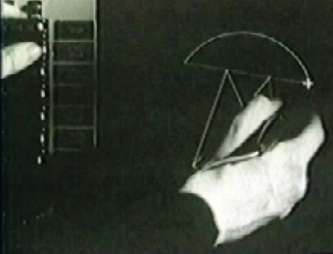
\includegraphics[width=\linewidth]{gfx/ellisSketchpad}}
	\caption[Sketchpad \newline \citep{Johnson:2009}]{Sketchpad unterstützt Benutzer beim Erstellen von Designzeichnungen mittels Stift (rechte Hand) und verschiedener Modi/Bedingungen (erreichbar über die Knöpfe auf der linken Seite).}
	\label{fig:ellisSketchpad}
\end{figure}

\begin{figure}
        \myfloatalign
        \subfloat[Input]
        {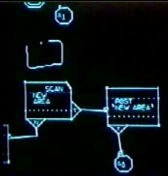
\includegraphics[width=.48\linewidth]{gfx/ellisGRAILinput}} \quad
        \subfloat[Output]
        {\label{fig:ellisGRAILinput}%
         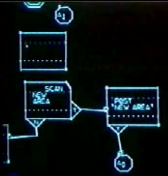
\includegraphics[width=.48\linewidth]{gfx/ellisGRAILoutput}} \\
        \caption[GRAIL Funktionalität \newline \citep{Johnson:2009}]{GRAIL analysiert die Benutzereingaben (a) und errechnet automatisch die bestimmungsgemäße Information (b) - hier z.B. ein Rechteck.}\label{fig:ellisGRAILoutput}
\end{figure}

\medskip Im \emph{GRAIL}\footnote{RAND's GRAIL (GRAphical Input Language) System aus dem Jahr 1968, interpretierte Stifteingaben in einer besonderen visuellen Programmiersprache, um Flussdiagramme zu erstellen \citep{Ellis:1969}. Benutzer konnten via Eingabetablet semantisch wertvolle Modelldaten (Rechtecke, Pfeile, Schrift) und Kommandos (Lösche eine Linie, Bewege ein Rechteck, etc.) zeichnen und GRAIL errechnete anschließend automatisch die bestimmungsgemäße Information.} System können Benutzer nicht explizit in einen anderen Modus wechseln, um Text und Grafiken zu bearbeiten. Stattdessen versucht das System die Absichten des Benutzers aus einer Analyse des Gezeichneten bzw. dessen Kontext zu erschließen (siehe \autoref{fig:ellisGRAILoutput}) \citep{Ellis:1969}. 

\medskip Diese zwei früh entwickelten Systeme stellen zwei Extreme gegenüber, die zeigen wie man mit dem Modusproblem umgehen kann. Sketchpad's Ansatz baut auf explizite Modiwechsel abseits des Stiftes auf - GRAIL's Ansatz auf implizite Modiwechsel, errechnet durch Stifteingaben.

\medskip Es scheint keinen >>richtigen<< Weg geben, um dem Modusproblem entgegenzuwirken. Implizite Modiwechsel scheinen natürlicher, aber nur wenn das System die Benutzereingaben richtig interpretiert. Interpretationstechniken sind fehleranfällig. Viele Systeme ermöglichen deswegen eine Kombination dieser zwei Arten oder verhängen Zeichenkonventionen.

\medskip Saund and Lank erforschten automatische Interpretationen und Modiwechsel, basierend auf Eingaben von Benutzern und bereits Gezeichneten \citep{Saund:2003p66}. Ihr \emph{Inferred-Mode Protocol} beschreibt einen Ansatz zur Analyse des Gezeichneten, um herauszufinden ob Aktionen mit Absicht durchgeführt wurden, oder nicht. War eine Aktion unklar, wird ein Mediator eingesetzt, der Methoden vorschlägt, um die Unklarheit zu beseitigen.

\medskip Li et al. verglichen in \citep{Li:2005} verschiedene Moduswechseltechniken für stiftbasierende User Interfaces. Dabei wurden folgende Techniken miteinbezogen: 
\begin{itemize}
	\item Tasten am Stift,
	\item Drücken und Halten,
	\item Benutzung der schwachen Hand um einen physikalischen Button zu drücken,
	\item ein neue durckbasierte Methode, und
	\item Benutzung des >>Radierers<< des Stiftes
\end{itemize}

Interessanterweise, \graffito{Explizite Modiwechsel durch physikalische Buttons sind die schnellsten, am Fehler unanfälligsten und beliebtesten.}war die Methode, in der die schwache Hand verwendet wurde die schnellste, am Fehler unanfälligsten und die beliebteste. Die >>Drücken und Halten<< Methode, wurde auch von Schilit et al. \citep{Schilit:1998} verwendet, die dies auch >>Rast<<-Geste bezeichneten. Microsoft Windows for Tablet PCs benutzt diese Geste beispielsweise um die Rechtsklick-Kontextmenüs aufzurufen.

\medskip Bei Skizziersystemen tritt das Modusproblem vorwiegend auf, da es mehrere Typen an Stifteingaben gibt. Manche Eingaben sollen auf einer Seite angezeigt werden, da sie Wörter, Zeichnungen oder andere Modellelemente (\emph{Model Operations}) darstellen, andere sollen im Hintergrund weiterverarbeitet werden, da sie Selektionen oder Kommandos (\emph{Environment Operations}) angeben.

\medskip \emph{Flow Selection} \citep{Johnson:2006} erlaubt Benutzern mit Hilfe der Rast-Geste nahtlos vom Zeichen- zum Selektionsmodus zu wechseln. Anschließende Operationen, wie Verschieben eines Teilabschnitts einer Linie, werden durch Bewegung des Stiftes ausgeführt -- ohne den Stift vorher abzusetzen. Wieviel Einzelpunkte vom darunter liegenden Objekt selektiert werden - man spricht dabei auch von der Selektionstärke - hängt vom Abstand zur Stiftposition ab und wie lange der Benutzer den Stift an der selben Stelle ruhen lässt. Die Selektionstärek wird bei Operationen wie Verschieben oder Glättung verwendet (vgl. \autoref{fig:johnsonFlowSelection3}).

\begin{figure}
        \myfloatalign
        \subfloat[ ]
        {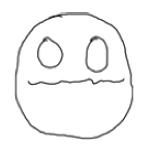
\includegraphics[width=.22\linewidth]{gfx/johnsonFlowSelection1}} \quad
        \subfloat[ ]
        {\label{fig:johnsonFlowSelection1}%
         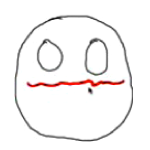
\includegraphics[width=.22\linewidth]{gfx/johnsonFlowSelection2}} \quad
		\subfloat[ ]
        {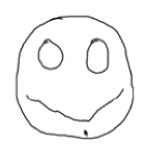
\includegraphics[width=.22\linewidth]{gfx/johnsonFlowSelection3}} \quad
        \subfloat[ ]
        {\label{fig:johnsonFlowSelection2}%
         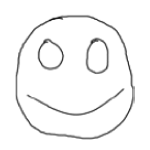
\includegraphics[width=.22\linewidth]{gfx/johnsonFlowSelection4}} \quad
        \caption[Modiwechsel \newline \citep{Johnson:2009}]{Modiwechsel der Flow Selection geschehen durch Halten und Bewegen des Stiftes \citep{Johnson:2006}. Der Benutzer positioniert dazu den Stift am gewünschten Objekt (a), bewegt es (b) ohne dabei den Stift zu heben (c). Der Benutzer hält den Stift anschließend an der Position bis die Kurve geglättet wurde (d) bevor er den Prozess durch heben des Stiftes abschließt.}\label{fig:johnsonFlowSelection3}
\end{figure}

\section{Die Bedeutung von Gestik}\label{sec:Gestik}

\begin{quote}
	\begin{flushright}{\slshape    
	    Design is an “activity of the mind \ldots grounded in mechanisms that evolved for interaction with the environment”.} \\ \medskip
	    --- \defcitealias{Wilson:2002}{M. Wilson}\citetalias{Wilson:2002} \citep{Wilson:2002}
	\end{flushright}
\end{quote}

Die Kombination von Gesten und Sprache bilden die Grundlage zur menschlichen dialogorientierten Interaktion. Wie man sich vorstellen kann, sind sie somit auch ein wichtiger Bestandteil von Design (vgl. obiges Zitat von Wilson). Um diese Modalitäten auch richtig in \ac{HCI} anwenden zu können, müssen wir ihre Wechselwirkung zur Kommunikation verstehen.

\medskip Was sind eigentlich Gesten? Wenn ein Student mit einer Krawatte in die Klasse kommt und der Professor keine trägt, geben beide eine Aussage über ihre Einstellung zu der Klasse ab - ob sie wollen oder nicht. \\ Solche Handlungen nennt man auch >>Nonverbale Kommunikation<<. Ein breites Spektrum an Verhaltensweisen zählt zu nonverbaler Kommunikation: die Wohn- und Arbeitsumgebungen, die wir schaffen; den Abstand, den wir zwischen uns und unseren Gegenüber einnehmen; ob wir unseren Körper bewegen, Augenkontakt herstellen, oder unsere Stimme erheben; all dies spielt zusammen und sendet Signale aus. \\
Die traditionelle Sicht auf Kommunikation teilt sich in die verbale und nonverbale Komponente, bzw. ihr Zusammenspiel. Adam Kendon (1980) war einer der ersten, der sich mit dieser Ansicht beschäftigte. Er behauptet, dass sich mindestens eine Form des nonverbalen Verhaltens - Gestik - von einer Konverstation nicht trennen lässt. David McNeill zeigte 1992 in seinen bahnbrechenden Studien über Gestik und Sprache, dass Handbewegungen, die wir beim Sprechen produzieren, fest mit dem Gesprochenen, bezüglich Timing, Bedeutung und Funktion verstrickt sind. Wenn man Gestik ignoriert, ignoriert man einen Teil der Konversation.

\medskip Gestik ist ein Begriff, der für einen großen Bereich steht. Betrachtet man z.B. lediglich Handbewegungen, kann man nicht einmal von einer eigenen Kategorie sprechen. \citep{Goldin:2003} \\ Ekman und Friesen veröffentlichten 1969 einen Entwurf um nonverbales Verhalten zu klassifizieren und identifizierten dabei fünf Typen:
\begin{itemize}
	\item \emph{Illustratoren}, dies sind Verhaltensweisen, die das Gesagte untermalen, illustrieren oder verdeutlichen;
	\item \emph{Adaptoren}, dies sind Verhaltensweisen, die der Erregungsabfuhr oder der Selbststimulierung dienen können;
	\item \emph{Emblemen}, dies sind Verhaltensweisen, die das gesprochene Wort ersetzen;
	\item \emph{Regulatoren}, dies sind Verhaltensweien, die Interaktion steuern;
	\item \emph{Affektdarstellungen}, dies sind Verhaltensweisen, die Affekte, Stimmungen und Emotionen ausdrücken.
\end{itemize} \begin{flushright} \citep{Schaefer:2003} \end{flushright}

Im folgenden beschäftigen wir uns mit einer dieser fünf: Illustratoren - auch \emph{Gestikulation} von Kendon (1980) und \emph{Gestik} von McNeill (1992) genannt. All diese Begriffe beschreiben Handbewegungen, die im direkten Bezug zu Gesprochenen stehen. Diese können das Tempo einer Rede vorgeben, auf Referenten verweisen, oder symbolischen Charakter haben um den Inhalt einer Rede zu verdeutlichen. \citep{Goldin:2003}

\medskip Bezüglich Skizzen ermöglicht es Gestik Meetingteilnehmer Details zu Zeichnungen zu erklären und zu interpretieren. Zusätzlich können hypothetische Modifikationen vorgenommen werden. Gestik bietet einen Mechanismus um Aktivitäten, Größen, Verbindungen, Richtungen oder Blickrichtungen zu kommunizieren. 
\\ Dantec schildert in \citep{Dantec:2009} die Erfahrungen, die er in einem Architekturdesignmeeting mit Gestik gemacht hat. \graffito{Gesten sind das primäre Mittel um Designprobleme zu lösen.} Über das gesamte Meeting hinweg waren Gesten das primäre Mittel um Designprobleme zu lösen. Trotz der unbeständigen Natur von Gesten, wurden sie wiederholt und effektiv eingesetzt um komplexe Konzepte zu kommunizieren, ohne zuvor ein spezielles Training absolviert zu haben. Die Effektivität von Gesten und die Art wie sie zwischen allen Teilnehmer fungierten, zeigte wie mehrere Teilnehmer mit eigenen Spezialisierungen ein verständliches Kommunikationsmittel fanden und so zum gemeinsamen Design beitrugen.

\medskip In Dantecs beschriebenen Szenario wurden Gesten auch dazu verwendet, um über Merkmale von Designs zu sprechen, die im zweidimensionalen Design nicht eindeutig hervorgingen. So machte z.B. ein Teilnehmer große schwungvolle Gesten um die Form und Platzierung kleiner Fenster in einer Kapelle zu beschreiben (siehe \autoref{fig:dantecGestures}). Die Gesten zeigten mit der Hilfe von den Skizzen ein klares Bild von Form und Größe, boten zudem aber noch mehr. Sie beinhalteten eine metaphorische Qualität, da sie ausdrücken konnten wie der Raum Ruhe erzeugt. Somit bekräftigten sie den Zweck des Gebäudes, der als Ort der Trauer gilt (siehe \extref{ext:dantecGestures}). Die Tatsache, dass die Nutzung von Gesten, physikalische Eigenschaften und metaphorische Qualitäten beschreiben kann, bestätigen auch die Forschungsergebnisse von Casasanto und Lozano, die die Rolle von Gesten beim Erarbeiten von abstrakten Konzepten untersuchten \citep{Casasanto:2006}.

\medskip Obwohl Gesten typischerweise nicht als Medium gesehen werden, die Informationen speichern (da sie keine permanenten Spuren hinterlassen), fanden Tang \& Leifer in \citep{Tang:1988p279} einen Beweis, dass Gesten Informationen effektiv in Stücke zerteilen und ins Gedächtnis zurückrufen können - insbesondere wenn die Gesten von anderen nachgeahmt oder schriftlich bzw. skizzenhaft zu Papier gebracht werden. In einer Designstudie beobachteten sie diesen Umstand. Durch Nachahmung einer Geste und dessen Benennung mit der Phrase >>slide and tap<<, blieb eine Idee in den Köpfen der Teilnehmer verankert.

\medskip In der selben Studie wurden diese und auch andere Funktionen von Gesten beobachtet und statistisch erfasst. Das gerade erwähnte Funktion \emph{Speichern von Information} wurde einmal verzeichnet, das \emph{Verdeutlichen von Ideen} 24 mal, \emph{Hinweisen auf Ideen} neun mal und \emph{Aufmerksamkeit erlangen} 46 mal (vgl. \autoref{fig:tangStatistik}). Wie man durch die Statistik erkennen kann, spielen Gesten eine wichtige Rolle in kollaborativen Situationen, da sie hauptsächlich dazu benutzt werden um anderen Personen Aktionen zu demonstrieren und die Aufmerksamkeit auf bestimmte Orte zu lenken.

\medskip Tang \& Minneman konzentrierten sich in \citep{Tang:1991p28} auf die Benutzung von Handgesten in Verbindung mit Zeichnungen. Handgesten treten oft in Verbindung mit Skizzen auf, um Informationen zu verdeutlichen. Aus diesem Grund entwickelten sie VideoDraw, ein kollaboratives Skizziersystem, das das Zusammenspiel von Skizzen und Gesten unterstützt. Das VideoDraw Setup besteht aus zwei Videokameras, die die Arbeitsflächen der Teilnehmer aufnimmt und direkt an den jeweilig gegenüberliegenden Bildschirm überträgt (vgl. \autoref{fig:tangVideoDraw}). Die Bildschirme fungieren als Whiteboard, auf das jeder Teilnehmer direkt mit Marker zeichnen kann. Die Zeichnungen \emph{und} Handgesten der Teilnehmer werden somit durch die Kamera erfasst und zum anderen Teilnehmer übertragen.

\medskip Handgesten können in VideoDraw beispielsweise eingesetzt werden, um einem Teilnehmer die geplante Bedienung eines User Interfaces zu erklären. Die Effektivität dieser Art von Gesten hängt von der Aufrechterhaltung der Verbindung zwischen den Händen und den Skizzen am VideoDraw Screen ab.

\medskip
\begin{figure}[bth]
	{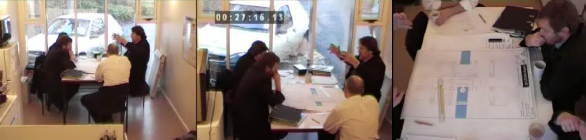
\includegraphics[width=\linewidth]{gfx/dantecGestures}}
	\caption[Beispiel von Gestik in einem Designmeeting. \citep{Dantec:2009}]{Ein Teilnehmer gestikuliert um Gebäudemerkmale zu beschreiben.}
	\label{fig:dantecGestures}
\end{figure}

\begin{extract}[Transkript eines Designmeetings. Skizzen und Gestik dienen als Ausdrucksmittel.]{
		\myfloatalign
		\begin{tabularx}{\textwidth}{p{1cm}X}
    		Adam & that wasn’t the idea I was anticipating that the hearses would be parked here [sketches] \\
			Anna & were there OK that’s fine yeah \\
			Adam & exactly as they are at the moment that the coffin would be drawn out	here and they would simply [points] walk it in I wasn’t thinking that they’d try and park \\
			Anna & no that’s OK \\
			Adam & in there \\
			Anna & yes well that’s what they’re wondering how that would work then so we’d work I wasn’t quite aware \\
			Adam & we’d work it exactly the same way as the present system I mean maybe this should be made more obvious by perhaps a different colour in the paving or something [sketches] I mean what I’m trying to say here is that that’s the vehicular line [sketches] \\
			Anna & yes \\
			Adam & and that these areas [points] are for people to mill about in and you’ve got a place for people to stand \\
			Anna & yes they will probably want to know how [points] how + how far that is from the because they’re going to be possibly carry the coffins in and most of the men are sort of in their seventies and eighties [laughs] carrying the coffin \\
		\end{tabularx}
	}
	\captionX{Gestik in Designmeetings.}
	\label{ext:dantecGestures}
\end{extract}

\begin{figure}[bth]
	{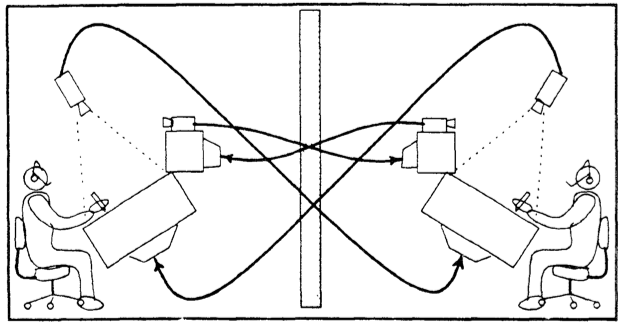
\includegraphics[width=\linewidth]{gfx/tangVideoDraw}}
	\caption[VideoDraw \newline \citep{Tang:1991p28}]{Schematische Darstellung von VideoDraw in einem Zwei-Personen-Szenario an verschiedenen Orten.}
	\label{fig:tangVideoDraw}
\end{figure}

%instead of newpage use \\[4cm]
\newpage Zusätzlich übermittelt VideoDraw auch Gesten mehrerer Hände und/oder Finger. Diese Kommunikation der Gesten ist reichhaltiger als die der meisten Computersysteme (typischerweise stellen diese lediglich einen mausgesteuerten Cursor zu Verfügung). VideoDraw überträgt ebenso das Gefühl von Dreidimensionalität.
Benutzer verfügen über >>räumliche<< Gesten und können sogar alltägliche Gegenstände ins Kamerabild holen, wodurch eine dreidimensionale Wahrnehmung von Raumverhältnissen den anderen Teilnehmern vermittelt werden kann.

\medskip Durch Observationen von Tang \& Minnemans System ließen sich vier Hauptmerkmale zusammenfassen.

\medskip VideoDraw:
\begin{itemize}
	\item übermittelt Handgesten unter den Teilnehmern;
	\item verursacht keine problematischen Verzögerungen in der Interaktion;
	\item bietet eine neuartige Wahrnehmung von räumlichen Beziehungen zwischen den Teilnehmern und ihrer Zeichenoberfläche; und
	\item erlaubt mehreren Teilnehmern gleichzeitiges Arbeiten auf der gleichen Arbeitsfläche.
\end{itemize}

VideoDraw erlaubt Teilnehmer gewohnte Tätigkeiten auf eine neue Art zu erleben. Es ermöglicht Benutzern ihre Zeichenoberfläche mit anderen Teilnehmern am selben oder an einem anderen Ort zu teilen - ohne dass dabei Verwirrungen in der Interaktion entstehen. Es ermöglicht zudem die Hände der Teilnehmer näher aneinander zubringen, als es in der Realität je möglich wäre - ohne die Teilnehmer gegenseitig zu behindern. \citep{Tang:1991p28}

\section{Case Study - Digital and Paper Media}

2010 führten Hinckley et al. eine Studie durch, in der sie mittels Observationen herausfinden wollten, wie Personen mit Papier, Stiften und Hilfsmittel arbeiten. Sie stellten den Probanden die Aufgabe, Ideen zu einem hypothetischen Kurzfilm zu illustrieren. Zu Verfügung standen ihnen Notizblöcke, Scheren, Stifte, Klebeband und 20 Seiten an inspirierenden Material. Acht Personen nahmen an der Studie teil und unterstützten so Hinchley et al. auf der Suche nach Verhaltensmustern in Sachen Gestik und Arbeitsplatzstrukturierung. Neun Verhaltensweisen (V\itshape 1\upshape-V\itshape 9\upshape) stachen besonders hervor:

\medskip \begin{enumerate}[V\itshape 1\upshape)]
	\item Teilnehmer klemmten den Stift zwischen die Finger der starken Hand, wenn sie vom Schreiben zum Schnipselverschieben wechselten (\hyperref[fig:hinckleyPaperNotebook]{Abbildung \ref*{fig:hinckleyPaperNotebook}a}).
	\item Teilnehmer hielten Schnipsel mit einem Finger der schwächeren Hand an einer Stelle (\hyperref[fig:hinckleyPaperNotebook]{Abbildung \ref*{fig:hinckleyPaperNotebook}a}).
	\item Teilnehmer tendierten dazu, Schnipsel mit der schwächeren Hand festzuhalten, wenn sie darauf schrieben (\hyperref[fig:hinckleyPaperNotebook]{Abbildung \ref*{fig:hinckleyPaperNotebook}b}).
	\item Eine häufig eingesetzter Handgriff war das Halten eines Schnipsels mit Daumen und Zeigefinger während dem Schreiben (\hyperref[fig:hinckleyPaperNotebook]{Abbildung \ref*{fig:hinckleyPaperNotebook}b}).
	\item Teilnehmer benutzten nur Teile des inspirierenden Materials. Sie schnitten Schnipsel über dem Notizblock indem sie das Material mit der schwächeren Hand hielten und die stärke Hand zuschnitt (\hyperref[fig:hinckleyPaperNotebook]{Abbildung \ref*{fig:hinckleyPaperNotebook}c}).
	\item Teilnehmer schoben das Notizbuch nahe zu ihrem Körper wenn sie zu den darüber liegenden Hilfsmittel fassten (\hyperref[fig:hinckleyPaperNotebook]{Abbildung \ref*{fig:hinckleyPaperNotebook}d}).
	\item Das Anhäufen von Schnipsel war ein häufiges Verhalten. Benutzer formten Stapel aus >>interessanten<< Objekten, während sie die übrigen in der schwächeren Hand hielten.
	\item Einige missbrauchten Schnipsel als Schablone, um einen Rahmen um ein Objekt zu zeichnen (\hyperref[fig:hinckleyPaperNotebook]{Abbildung \ref*{fig:hinckleyPaperNotebook}e}).
	\item Das Reißen von Papier war eine zweihändige Arbeit, die mit den Fingern vollzogen wurde (\hyperref[fig:hinckleyPaperNotebook]{Abbildung \ref*{fig:hinckleyPaperNotebook}f}).
\end{enumerate}

\begin{flushright} \citep{Hinckley:2010} \end{flushright}

\begin{figure}[bth]
	{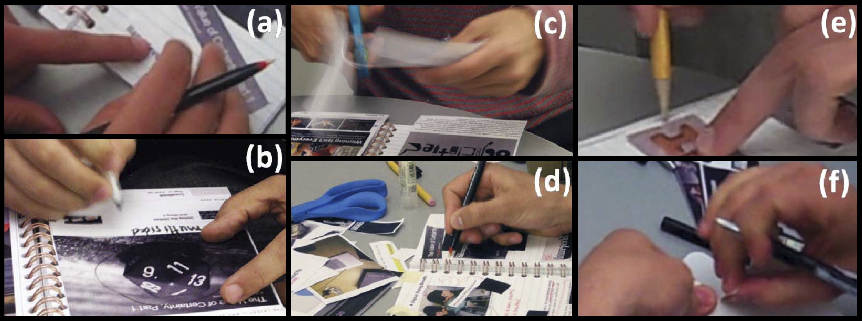
\includegraphics[width=\linewidth]{gfx/hinckleyPaperNotebook}}
	\caption[Designstudie über die Benutzung von Notizbüchern \newline \citep{Hinckley:2010}]{Verhaltensweisen bei der Benutzung von Notitzbüchern. \begin{inparaenum}[\itshape a\upshape)] \textbf{\item} Benutzer klemmen Stifte zwischen ihre finger, während sie Objekte bearbeiten. \textbf{\item} Daumen und Zeigefinger halten ein Objekt fest, während darauf geschrieben wird. \textbf{\item} Papierschnipsel fallen auf die Arbeitsfläche. \textbf{\item} Benutzer greifen oft nach Hilfsmitteln und neuen Inhalten, die über dem Notizbuch liegen. \textbf{\item} Zeichnen eines Rahmens mit einer Schablone, durch Halten der Schablone mit der Hilfshand und Nachfahren der Kanten mit dem Stift. \textbf{\item} Reißen einer Seite durch Festhalten des Papiers mit dem Daumen und Ziehen mit den Fingern der anderen Hand. Der Stift ist währenddessen wiederum zwischen den Fingern eingeklemmt. \end{inparaenum}}
	\label{fig:hinckleyPaperNotebook}
\end{figure}

Piper \& Hollan suchten im Weiteren den direkten Vergleich von Papier zu digitalen Medien und starteten dazu eine Untersuchung, in der sie Paare von Studenten mit Papier und digitalen Materialien auf Tabletop-Umgebungen arbeiten ließen. Die digitale Umgebung umfasste ein Tabletop-Display (vgl. \hyperref[fn:tableTop]{Fußnote \ref*{fn:tableTop}} in \autoref{sec:groupWareTools}) mit einer \emph{\ac{SDG}}\footnote{Single Display Groupware (\ac{SDG}) ist eine Spezialform von Groupware (vgl. \nameref{ch:CSCWDesign}) und beschreibt eine Displaytechnologie, die Eingaben von mehreren Benutzern gleichzeitig unterstützt \citep{Stewart:1997}. \ac{SDG}Ï führt zu höherem Engagement und gerechteren Aufgabenteilung \citep{Stewart:1999}.} - die andere enthielt Papier, Hilfsmittel und einen Tisch.

\medskip 20 Studenten einer neurowissenschaftlichen Einführungslehrveranstaltung nahmen fünf Wochen an der Untersuchung teil. Die Studenten mussten mit den vorgegebenen Systemen arbeiten und am Ende der Lehrveranstalung in der Lage sein, die Anatomie des Gehirnes aufzusagen, komplexe Systeme (wie z.B. die Entladung einer Nervenzelle) zu verstehen und zu beschreiben, sowie verschiedene Graphen und Schaltungen von Gehirnaktivitäten zu erstellen. Jede Teiluntersuchung umfasste folgende drei, vom Professor ausgewählte, Aktivitäten:
\begin{enumerate}
	\item das Beschriften der Gehirnanatomie,
	\item das Auseinandersetzen mit einem dynamischen System, und
	\item das Zeichnen eines Graphen oder einer Schaltung.
\end{enumerate}
Das Ziel jeder Teiluntersuchung war die Studenten auf ein kommendes Examen vorzubereiten. Die Arbeitsmittel beider Gruppen (analog, sowie digital Arbeitende) wurden soweit wie möglich angeglichen. Lediglich die Größe der Arbeitsfläche unterschied sich von der 79cm langen Bildschirmdiagonale zu den ca. 35cm Diagonale eines Blatt Papiers im A4 Format.

\medskip Papier- und Digitalmedien haben einzigartige und ergänzende Merkmale für kleine Lerngruppen. Die Studenten, die mit Papiermaterialen gearbeitet haben, machten detaillierte Notizen und erarbeiteten meist ernsthaftere Arbeitsstrategien. Auf der anderen Seite diskutierten die Studenten, die am Tabletop-Display arbeiteten, ihre Ideen bevor sie sich die Antworten ansahen, wiederholten Aktivitäten und schnitten besser im Endexamen ab. \citep{Piper:2009}
\\Während die folgenden Ergebnisse der Studie auf die Aktivitäten von Lerngruppen ausgelegt sind, können trotzdem auch allgemeine kognitive und soziale Merkmale, in Bezug auf die Arbeit in beiden Welten (traditionell \& digital), entnommen werden.

\subsection{Kognitive Merkmale}
Papier ist das traditionelle Medium für Schulungsunterlagen. In Lerngruppen interagieren Studenten üblicherweise mit Papierdokumenten. Dadurch, dass die Teilnehmer der Studie keine vorgehende Erfahrung mit einem kollaborativen Tabletop Umgebungen hatten, hatten sie anfangs geringe Schwierigkeiten sich an das System zu gewöhnen. Jedoch förderte die Neuheit des digitalen Mediums einen gewissen Freiraum zur Interaktion. Munter kritzelten die Studenten mit den digitalen Stiften darauf los, während der Enthusiasmus bei den Studenten, die mit den traditionellen Mitteln arbeiteten sich in Grenzen hielt. Ebenso, ermutigten der geringe Aufwand und die geringen Konsequenzen (wenn etwas falsches gezeichnet wird, kann es leicht wieder gelöscht werden) die Studenten spontan Zeichnungen zu erstellen um die Diskussion zu unterstützen. Diese spontanen Skizzen können den Lernprozess ebenso in kognitiver Art unterstützen; die Skizzen bieten eine externe Abbildung der Diskussionen und bieten eine Grundlage um ein Verständnis zu entwickeln. Studenten, die mit Papierdokumenten arbeiteten, waren eher dazu geneigt die vorgegebenen Diagramme zu wenden, um auf der Rückseite zu zeichnen, anstatt direkt auf dem Bild. Die digitalen Medien ermutigten die Studenten nicht nur direkt auf ein Diagramm zu zeichnen, sondern auch die Radierfunktion öfter einzusetzen. Notizen auf Papierdokumenten wurden weniger ausradiert. Dadurch konnten die Studenten, die mit Papier arbeiteten, zurück gehen und ihre alten Notizen und Skizzen durchsehen, was bei den digitalen Materialien oft nicht mehr möglich war. Natürlich muss dies nicht zwangsweise so ablaufen. Die Formbarkeit digitaler Medien erlaubt zahlreiche interessante Lösungsansätze. Die Möglichkeit digitale Annotierungen zu löschen führt zu kognitiven Folgen, die nähere Untersuchungen benötigen.

\medskip Digitale Tische können ebenfalls ein dynamischeres und umfassenderes Erlebnis ermöglichen, als traditionelle Papierdokumente. Das hat ebenso positive wie negative Konsequenten. Studien über das Lernen mit Diagrammen zeigen, dass digital animierte Diagramme Personen dazu zwingen das Diagramm wahrzunehmen, es richtig zuzuordnen und dann Diagrammänderungen durchzuführen, was zu einer höheren kognitiven Belastung führt, als statische Papierdiagramme \citep{Price:2002}. Andererseits ermöglichen große Touchscreens und interaktive Möglichkeiten, Formen an Interaktionen, die sich von den Papiermaterialen unterscheiden. Kognitionstheorien und die neuesten empirischen Forschungen zeigen, dass uns die körperliche Belastung hilft und zwingt abstrakte Konzepte zu verstehen \citep{Clark:1996,Johnson:1987,Nunez:1999,Varela:1991}. Das Zeichnen oder Nachverfolgen von Graphen mit dem Finger, ist ein konkreter kognitiver Prozess, der möglicherweise zu einem besseren Verständnis und Verinnerlichung eines abstrakten Konzeptes führt \citep{Goldin:2003}. \extref{ext:piperCognitiveAffordances} zeigt zwei Aussagen von Studenten, die mit digitalen Dokumenten arbeiteten. Piper \& Hollan glauben, dass konkrete Wahrnehmung eine zentrale Rolle im Verstehen kognitiver Askpekte im Zusammenhang mit Multitouchoberflächen spielen. \citep{Piper:2009}

\begin{extract}[Zwei typische Aussagen beim Arbeiten mit einem digitalen Tabletop-System.]{
		\myfloatalign
		\begin{tabularx}{\textwidth}{p{2cm}X}
    		Student D1 & Want to redraw it together to help memorize it? \\
			 & ... \\
			Student D2 & You want to try tracing it [the answer key]? It’s good practice. \\
		\end{tabularx}
	}
	\captionX{Arbeiten an digitalen Tabletop-Systemen.}
	\label{ext:piperCognitiveAffordances}
\end{extract}

\subsection{Soziale Merkmale}
Tabletop-Displays erlauben durch ihre Größe und ihre gemeinsame Nutzbarkeit, einen gleichmäßigen Zugang zu Materialen und erlauben gleichzeitiges Arbeiten. Aber verbessert dies den Lernprozess? Es gibt interessante Unterschiede zwischen den von Piper \& Hollan beobachteten parallelen Arbeitsweisen mit digitalen Dokumenten und seriellen Arbeitsweisen mit Papierdokumenten. Zum einen bedeutet paralleles Arbeiten, dass mehrere den gleichen und direkten Zugang zu Materialen haben - zum anderen kann dies aber dazu führen, dass man wichtige Teile der Aktivitäten bzw. des Problemlösungsprozess verpasst. Eine serielle Arbeitsweise hat ebenso positive und negative Auswirkungen auf den Lernprozess. Während sich beide Studenten gemeinsam auf eine Aufgabe konzentrieren, macht einer den Hauptteil der Arbeit. Der Partner nimmt eine passive Rolle an.

\medskip Idealerweise würde die Lernumgebung Studenten dazu bewegen, sich gleichermaßen zu beteiligen und den Fokus auf die Aufgabe zu richten. Tabletop-Technologien erlauben Unterrichtenden zumindest die Darstellung der Lehrmittel soweit zu verändern, damit soziale Barrieren vermieden werden und eine ausgeglichene Beteiligung herrscht. \citep{Piper:2009}

\section*{Zusammenfassung}
Traditionelle und digitale Medien haben unterschiedliche Stärken und Schwächen. Papierdokumente sind billig, portabel und perfekt geeignet um mit beiden Händen und einfachen Geräten wie Stiften daran zu arbeiten. Digitale Dokumente können hingegen mit Leichtigkeit editiert und schnell abgelegt bzw. abgerufen werden. Trotzdem kommt das Arbeiten mit einem strukturierten Softwaretool, nicht an die Schnelligkeit von unstrukturierten Papier-und-Stift Skizzen heran. \\
Um auf Computer ähnlich gut skizzieren zu können, wurden Eingabegeräte wie Tablets geschaffen. Die Interaktion mit Tabletstiften unterscheidet sich jedoch stark von der der Maus. Aus diesem Grund wurden eigene Interaktionstechniken für stiftbasierte Skizziersysteme entwickelt. Skizziersysteme besitzen auch oft mehrere Programmmodi um die Funktion der Stifte zu bestimmen. Dabei kommt es oft zu kognitiven Überlastungen bei den Benutzern, welche mit Hilfe einiger Strategien vermieden werden sollten. \\
Gestik ist ebenso ein wichtiger Faktor im kollaborativen Designprozess und kann bei digitalen Arbeitsweisen berücksichtigt werden. Weitere Faktoren und Eigenschaften von kollaborativen computerbasierten Systemen werden nun im nächsten Kapitel erläutert.